\documentclass[spanish, c, dvipsnames]{beamer}

\usepackage[utf8]{inputenc}
%\usepackage[spanish, mexico]{babel}
\usepackage{amsmath}
\usepackage{mathtools}
\usepackage{hyperref}
\usepackage{color}
\usepackage{xcolor}
\usepackage{ragged2e}
\usepackage{mathrsfs}
\usepackage{csquotes}
\usepackage{listings}
\usepackage[scaled]{beramono}
\usepackage[T1]{fontenc}
\usepackage{matlab-prettifier}
\usepackage{graphicx}
\usepackage{booktabs}
\usepackage{gensymb}
\usepackage{physics}
\usepackage{bigints}

\renewcommand{\indent}{\hspace*{2em}}

% \usepackage{tikz}

% \usetikzlibrary{fit, shapes, arrows}

% \usepackage{courier}
% \usepackage{subfigure}
% \usepackage{enumerate}
% \usepackage{algorithmic}
% \usepackage{algorithm}

% \usepackage{listings}
% \usepackage{lstlinebgrd}

\usetheme{Boadilla}
\usefonttheme[onlymath]{serif}

\newcommand{\matlab}[1]{\lstinline[style=Matlab-editor]!#1!}
\newcommand\blfootnote[1]{%
\begingroup
\renewcommand\thefootnote{}\footnote{#1}%
\addtocounter{footnote}{-1}%
\endgroup
}

\newcommand{\contrastA}[1]{{\color{red} #1}}
\newcommand{\contrastB}[1]{{\color{blue} #1}}

\lstset
{
    language = Matlab,
    style = Matlab-editor,
    basicstyle = \mlttfamily\scriptsize,
    escapechar = `,
    numbers = left,
    frame = tb,
}

\lstdefinestyle{output}
{
    language = {},
    basicstyle = \mlttfamily\scriptsize,
    escapechar = `,
    numbers = none,
    showtabs = false,
   	showstringspaces = false,
}

\makeatletter
\renewcommand*\env@matrix[1][*\c@MaxMatrixCols c]{%
  \hskip -\arraycolsep
  \let\@ifnextchar\new@ifnextchar
  \array{#1}}
\makeatother

% Sets the templates
\definecolor{navyblue}{RGB}{0, 0, 128}
\definecolor{crimson}{RGB}{128, 16, 0}

\setbeamertemplate{navigation symbols}{}
\setbeamertemplate{headline}{}
\setbeamertemplate{title page}[default][colsep=-4bp,rounded=true]
\setbeamertemplate{footline}[frame number]
\setbeamertemplate{bibliography item}[text]
\setbeamertemplate{theorems}[numbered]

\setbeamercolor{title}{fg=navyblue, bg=white}
\setbeamercolor{frametitle}{fg=navyblue, bg=white}
\setbeamercolor{structure}{fg=navyblue}
\setbeamercolor{button}{fg=white,bg=navyblue}

\setbeamercovered{transparent}

\title{Cálculo Numérico: Integrales numéricas}
\subtitle{Aplicación de Métodos Numéricos al Ambiente Construido \\ (CV1012)}
\author{
    \texorpdfstring{
        \begin{center}
            M.C. Xavier Sánchez Díaz \\
            \href{mailto:sax@tec.mx}{\texttt{sax@tec.mx}}
        \end{center}
    }
    {M.C. Xavier Sánchez Díaz}
}

\institute[Tecnológico de Monterrey]{
\includegraphics[scale=0.5]{../img/logo}}
\date{}

\begin{document}

\setlength{\rightskip}{0pt}

\begin{frame}[plain]
    \titlepage        
\end{frame}

\begin{frame}{Outline}
    \tableofcontents
\end{frame}

\section{Repaso de Cálculo}

\begin{frame}{La Derivada}{Repaso de Cálculo}
    \begin{itemize}
        \item Una \alert{derivada} $f'$ es una \textbf{operación} que toma como operando a una \textbf{función} $f$
        \item La derivada de una función $f$ en un punto $x_i$, hace referencia a la recta \textbf{tangente} que pasa por $x_i$
        \item La derivada es la \textbf{pendiente} de la tangente de dicha curva en el punto $x_i$
    \end{itemize}

    \begin{center}
        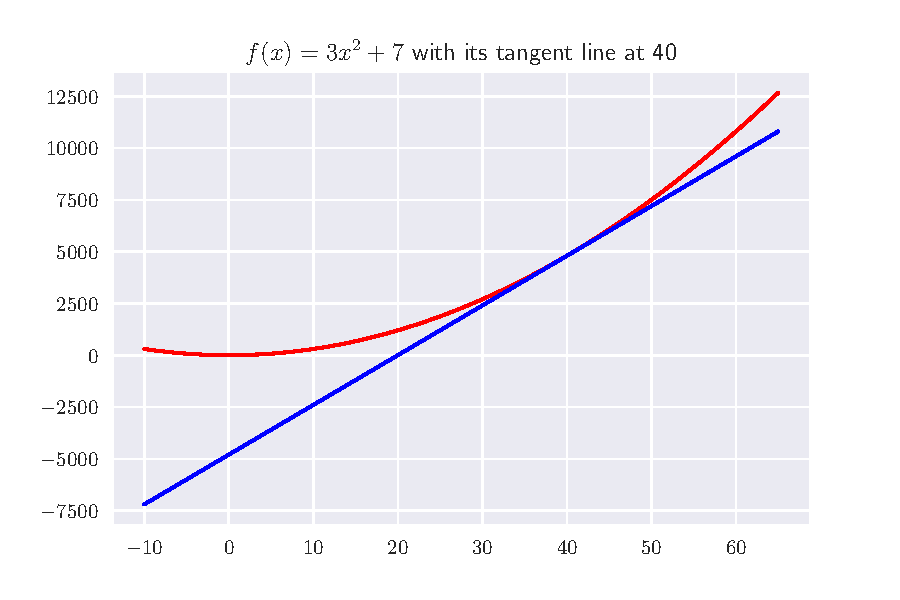
\includegraphics[width=0.5\textwidth]{tangent.pdf}
    \end{center}
\end{frame}

\begin{frame}{Derivada y Diferenciación}{Repaso de Cálculo}

    Como la \textbf{derivada} hace referencia a la \textbf{pendiente} de la recta tangente, nos está dando una medida de \alert{cambio}---cómo cambia la función en ese punto.

    \bigskip
    
    El cambio se puede \textbf{aproximar} usando diferencias.

    \begin{center}
        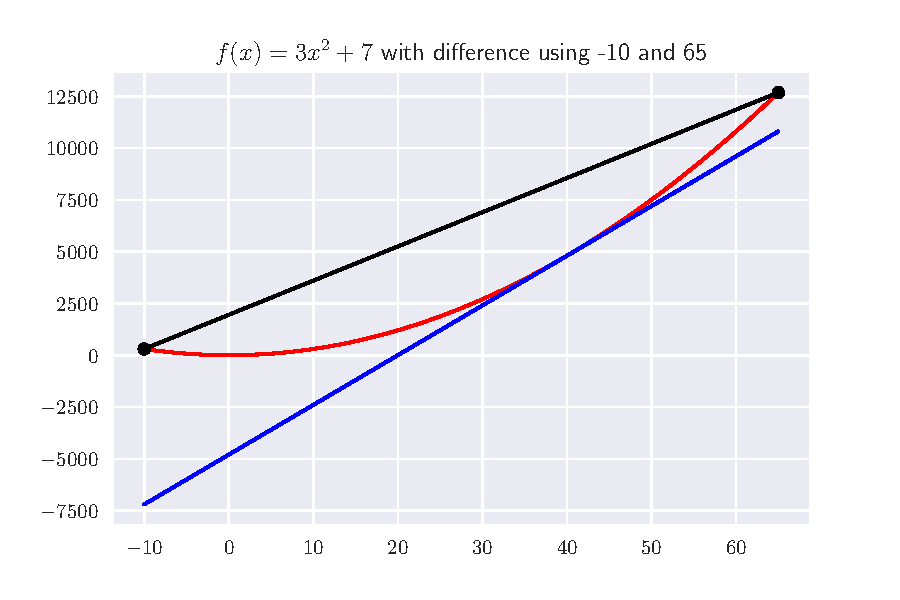
\includegraphics[width=0.5\textwidth]{diff01.pdf}
    \end{center}

\end{frame}

\begin{frame}{Derivada y Diferenciación}{Repaso de Cálculo}
    A medida que la diferencia se hace más pequeña, la aproximación de la derivada es mejor.

    \begin{center}
        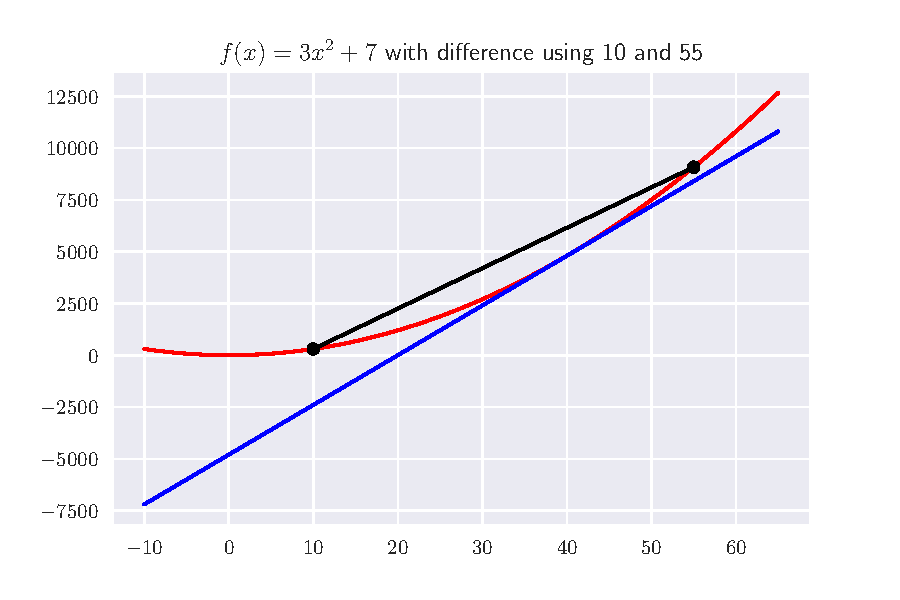
\includegraphics[width=0.5\textwidth]{diff02.pdf}
    \end{center}
\end{frame}

\begin{frame}{Derivada y Diferenciación}{Repaso de Cálculo}
    A medida que la diferencia se hace más pequeña, la aproximación de la derivada es mejor.

    \begin{center}
        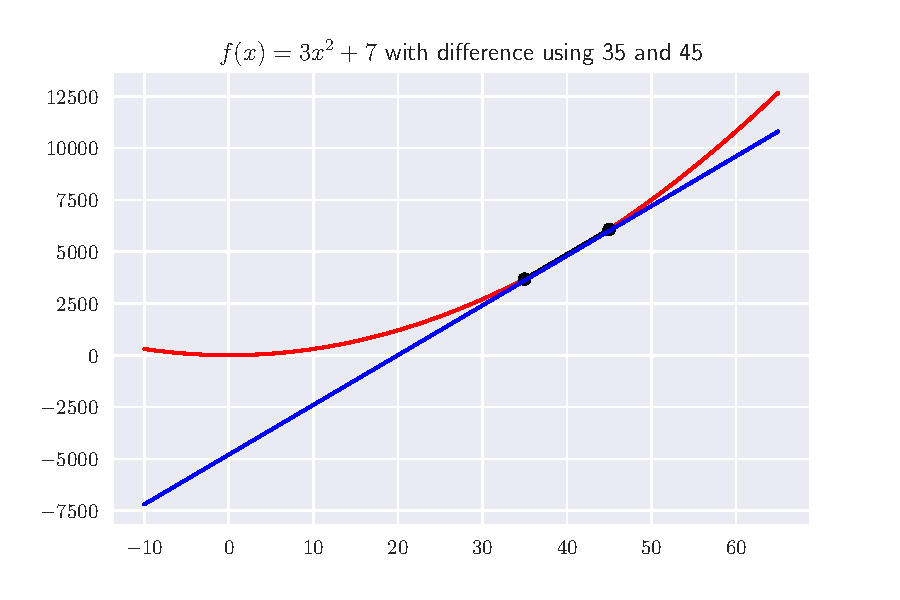
\includegraphics[width=0.5\textwidth]{diff03.pdf}
    \end{center}
\end{frame}

\begin{frame}{Integral}{Repaso de Cálculo}
    \begin{itemize}
        \item Una \alert{integral} $F$ es una \textbf{operación} que toma como operando a una \textbf{función} $f$
        \item La integral de una función $f$ es también conocida como su \textbf{antiderivada}, pues es la operación inversa a la derivada
        \item La integral de una función $f$ es la suma de todos los cambios que ocurren en una función $f$
    \end{itemize}

    \begin{center}
        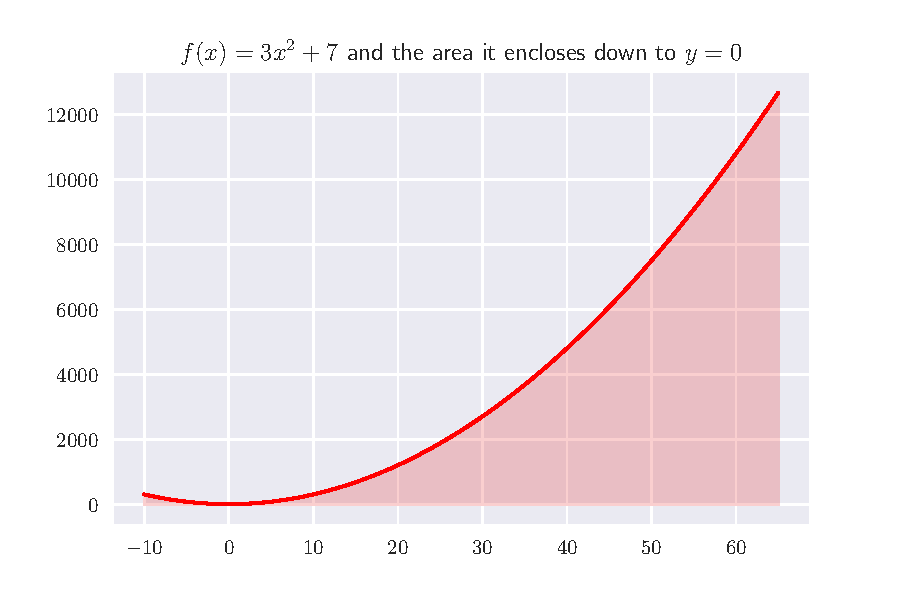
\includegraphics[width=0.5\textwidth]{area.pdf}
    \end{center}
\end{frame}

\begin{frame}{Integral y área bajo la curva}{Repaso de Cálculo}
    Como la \textbf{integral} hace referencia a la \alert{suma} de los cambios en cada uno de los puntos de la función, nos está dando una medida de agrupación---el área bajo la curva.

    Esta suma se puede \textbf{aproximar} definiendo pequeñas \textit{diferencias} y sumándolas.

    \begin{center}
        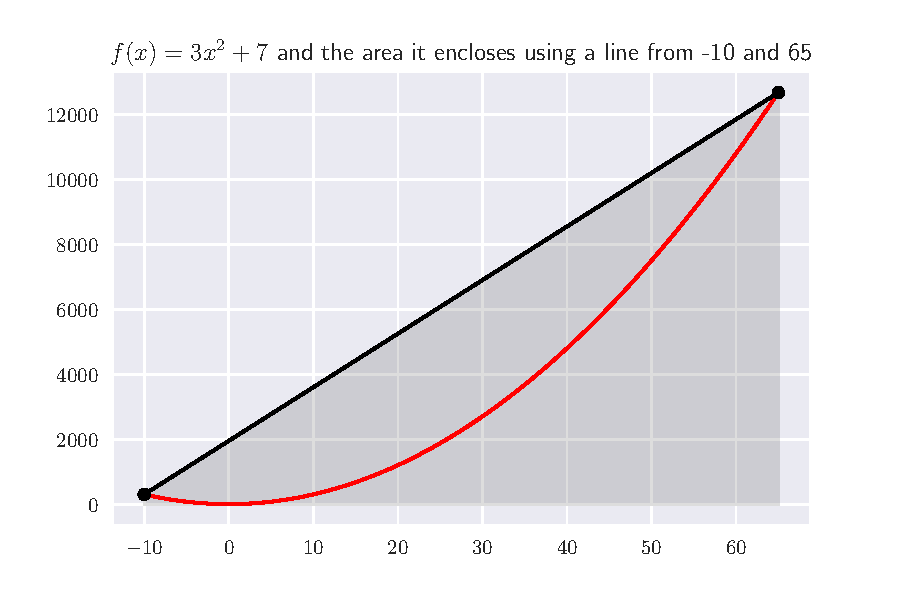
\includegraphics[width=0.5\textwidth]{int01.pdf}
    \end{center}    

\end{frame}

\begin{frame}{Integral y área bajo la curva}{Repaso de Cálculo}

    A medida que la diferencia se hace más pequeña, la aproximación del área bajo la curva es mejor.

    \begin{center}
        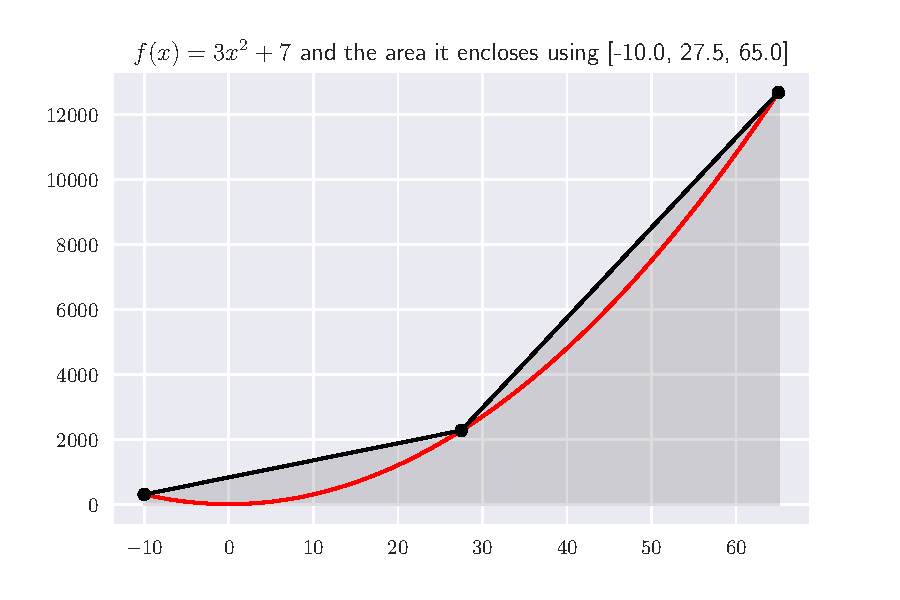
\includegraphics[width=0.5\textwidth]{int02.pdf}
    \end{center}    

\end{frame}

\begin{frame}{Integral y área bajo la curva}{Repaso de Cálculo}

    A medida que la diferencia se hace más pequeña, la aproximación del área bajo la curva es mejor.

    \begin{center}
        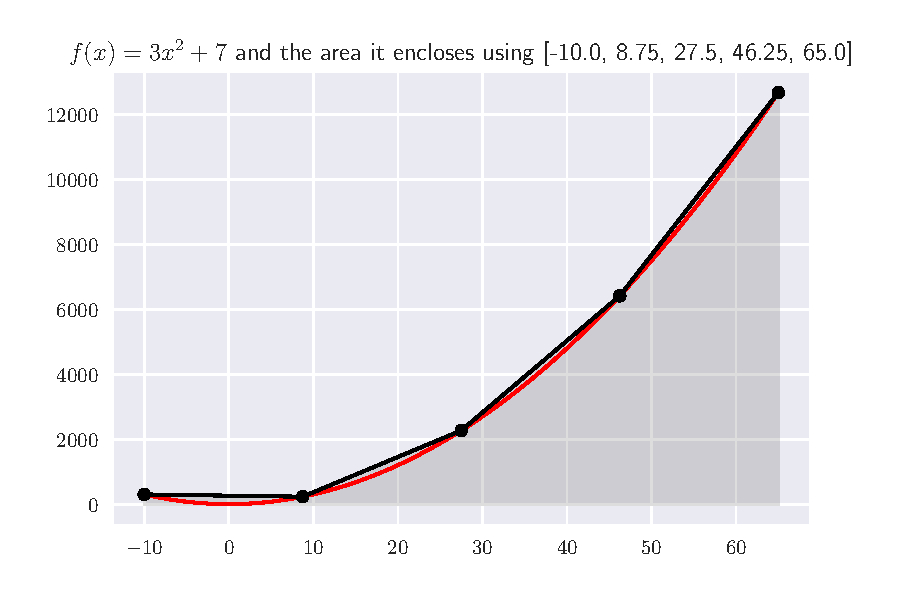
\includegraphics[width=0.5\textwidth]{int03.pdf}
    \end{center}    

\end{frame}

\section{Newton-Cotes}

\begin{frame}{Newton Cotes}{Integración Numérica}

    Las \textit{fórmulas} \alert{Newton-Cotes} son esquemas de integración numérica ampliamente usados.
    La idea se basa en reemplazar una función \textit{complicada} o datos tabulados con una función aproximada que sea más fácil de integrar.
    Por ejemplo:

    $$\int\limits_a^b f(x)\dd{x} \approx  \int\limits_a^b f_n(x)\dd{x}$$

    donde $f_n(x)$ es un \textbf{polinomio} de la forma

    $$f_n(x) = a_n x^n + a_{n-1} x^{n-1} + \dots + a_1 x + a_0$$
    
    y $n$ es el \textbf{orden} (o \textbf{grado}) del polinomio.

\end{frame}

\section{Regla del Trapecio}

\begin{frame}{Regla del Trapecio}{Newton-Cotes}

    La \alert{regla del trapecio} se refiere a la primera de las reglas de Newton-Cotes en intervalos cerrados (de $a$ a $b$, por ejemplo), y corresponde al caso donde el polinomio $f_n$ es de \alert{primer orden} $f_1$:

    $$\int\limits_a^b f(x)\dd{x} \approx  \int\limits_a^b f_1(x)\dd{x}$$

    que corresponde a la siguiente regla general

    \begin{block}{Regla del Trapecio}
        \begin{equation}
            \label{eq:trapezoidal-single}
            I = (b-a) \frac{f(a) + f(b)}{2}
        \end{equation}
    \end{block}
\end{frame}

\begin{frame}{Mejorando la aproximación}{Newton-Cotes}
    Para poder mejorar la aproximación usando la \textbf{regla del trapecio} podemos aplicarla en repetidas ocasiones: en lugar de usar un segmento, usar \alert{múltiples segmentos}.

    En este caso, tendremos que la integral numérica definida entre dos puntos $a$ y $b$ se puede calcular con la regla general siguiente:

    \bigskip

    \begin{block}{Aplicaciones múltiples de la regla del trapecio}
        \begin{equation}
            \label{eq:trapezoidal-multi}
            I = (b-a)\frac{f(x_0) + 2 \sum\limits_{i=1}^{n-1} f(x_i) + f(x_n)}{2n}
        \end{equation}
    \end{block}    

\end{frame}

\subsection{Cálculo del error en regla del trapecio}

\begin{frame}{Calculando el error de la regla del trapecio}{Newton-Cotes}
    Para calcular el \textbf{error} en la integral obtenida por la regla del trapecio \textbf{aplicada una vez}, podemos emplear la ecuación

    \bigskip

    \begin{block}{Error en la regla del trapecio}
        \begin{equation}
            \label{eq:trapezoidal-single-error}
            E_t = -\frac{1}{12} f''(\xi)(b-a)^3
        \end{equation}
    \end{block}

    \bigskip

    donde $\xi$ es un valor dentro del intervalo entre $a$ y $b$, y $f''$ es la segunda derivada de $x$. Después simplemente evaluamos en $\xi$.
\end{frame}

\begin{frame}{Calculando el error de la regla del trapecio}{Newton-Cotes}
    Si vamos a aplicarla múltiples veces, entonces necesitaremos sumar el error del intervalo en cada aplicación:

    \begin{block}{Error total en múltiples aplicaciones de la regla del trapecio}
        \begin{equation}
            \label{eq:trapezoidal-multi-error-exact}
            E_t = - \frac{(b-a)^3}{12 n^3} \sum\limits_{i=1}^n f''(\xi_i)
        \end{equation}
    \end{block}

    Se puede simplificar el cálculo si en lugar de sumar cada error, obtenemos el error para un \alert{intervalo promedio} aunque esto genera pérdida de precisión:

    \begin{exampleblock}{Error aproximado en múltiples aplicaciones de la regla del trapecio}
        \begin{equation}
            \label{eq:trapezoidal-multi-error-approx}
            E_a = - \frac{(b - a)^3}{12n^2} \alert{\bar{f''}}
        \end{equation}
    \end{exampleblock}

\end{frame}

\begin{frame}{Segunda derivada aproximada}{Newton-Cotes}
    Para calcular el valor de la \alert{segunda derivada promedio} cuando en lugar de tener mediciones discretas tenemos una función continua, podemos usar la siguiente aproximación:

    \bigskip

    \begin{block}{Aproximación de la segunda derivada promedio}
        \begin{equation}
            \label{eq:average-second-derivative}
            \bar{f''} = \dfrac{\bigint _a^b f''(x)}{b - a}
        \end{equation}
    \end{block}
\end{frame}

\begin{frame}{Ejercicio}{Aplicación múltiple de la Regla del Trapecio}
    \begin{center}
        Utiliza la regla del trapecio usando \textbf{dos segmentos} para estimar la integral definida de la función
        $$f(x) = 0.2 + 25x - 200 x^2 + 675 x^3 - 900 x^4 + 400x^5$$
        
        de $a=0$ a $b = 0.8$

        \bigskip

        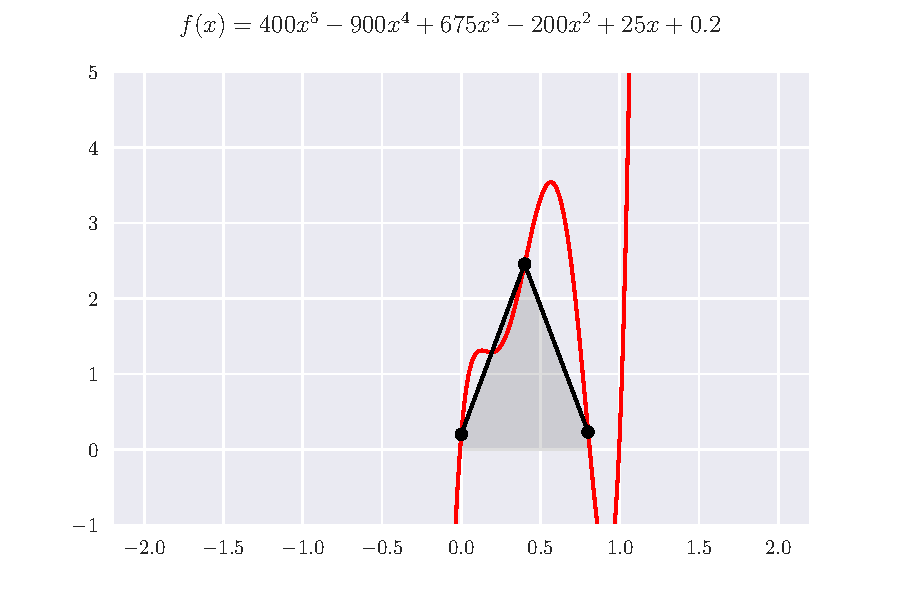
\includegraphics[width=0.5\textwidth]{two-segment.pdf}
    \end{center}
\end{frame}

\section{Regla de Simpson 1/3}

\begin{frame}{Integrando usando polinomios}{Newton-Cotes}
    Otra opción para poder aproximar una integral es usar \textbf{polinomios de mayor orden} para conectar los puntos.
    
    \bigskip

    Por ejemplo, para unir 3 puntos, podemos usar una \textbf{parábola}

    \bigskip

    \begin{center}
        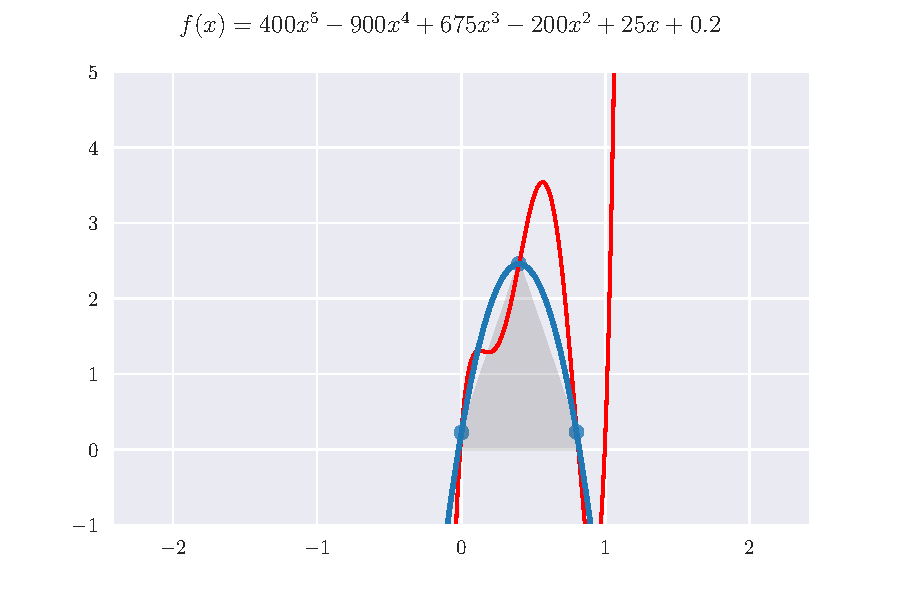
\includegraphics[width=0.5\textwidth]{simpsononethird.pdf}
    \end{center}

\end{frame}


\begin{frame}{Regla de Simpson 1/3}{Newton-Cotes}
    Específicamente, si usamos un polinomio de grado 2, es decir:

    $$\int\limits_a^b f(x)\dd{x} \approx  \int\limits_a^b f_2(x)\dd{x}$$

    \bigskip

    entonces estamos aplicando la \alert{regla de Simpson 1/3}, cuya ecuación general es:

    \bigskip

    \begin{block}{Regla de Simpson 1/3}
        \begin{equation}
            \label{eq:simpson13-single}
            I = (b-a) \frac{f(x_0) + 4 f(x_1) + f(x_2)}{6}
        \end{equation}
    \end{block}

\end{frame}

\begin{frame}{Múltiples aplicaciones de la regla de Simpson 1/3}{Newton-Cotes}

    Al igual que con la regla del trapecio, podemos aplicar varias veces la \textbf{regla de Simpson 1/3} para generar \alert{múltiples parábolas}.

    \bigskip

    En este caso, la integral numérica definida entre los puntos $a$ y $b$ puede aproximarse como sigue:

    \bigskip

    \begin{exampleblock}{Aplicaciones múltiples de la Regla de Simpson 1/3}
    \begin{equation}
        \label{eq:simpson13-multi}
        I = (b - a) \frac{f(x_0) + 4 \sum\limits_{i=1,3,5, \dots}^{n-1}f(x_i) + 2 \sum\limits_{j=2,4,6, \dots}^{n-2} f(x_j) + f(x_n)}{3n}
    \end{equation}
    \end{exampleblock}

\end{frame}

\begin{frame}{Múltiples aplicaciones de la regla de Simpson 1/3}{Newton-Cotes}
    \begin{center}
        $I = (b - a) \frac{f(x_0) + 4 \sum\limits_{\alert{i=1,3,5}}^{\alert{n-1}}f(x_i) + 2 \sum\limits_{\alert{j=2,4,6}}^{\alert{n-2}} f(x_j) + f(x_n)}{3n}$    
    \end{center}
    \bigskip
    Viendo de cerca la fórmula, podemos inferir que esta regla se puede usar sólo cuando tenemos un \alert{número par de segmentos}:
    \begin{center}
        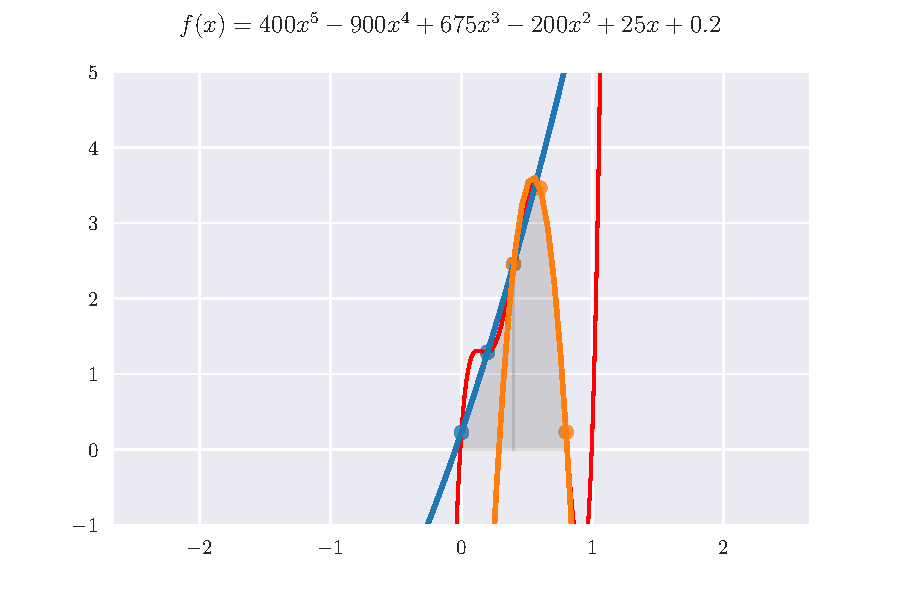
\includegraphics[width=0.5\textwidth]{simpsonmultionethird.pdf}
    \end{center}
\end{frame}

\begin{frame}{Calculando el error para la Regla de Simpson 1/3}{Newton-Cotes}
El error lo podemos calcular con las siguientes ecuaciones:

\begin{block}{Error total en aplicación singular de Regla de Simpson 1/3}
    \begin{equation}
        \label{eq:simpson13-single-error}
        E_t = - \frac{(b - a)^5}{2880}f^{(4)}(\xi)
    \end{equation}
\end{block}

donde $\xi$ es un valor dentro del intervalo entre $a$ y $b$, y $f^{(4)}$ es la cuarta derivada de $f(x)$. Después simplemente evaluamos en $\xi$.

\bigskip

\begin{exampleblock}{Error aproximado en aplicación múltiple de Regla de Simpson 1/3}
    \begin{equation}
        \label{eq:simpson13-multi-error}
        E_a = -\frac{(b - a)^5}{180 n^4} \bar{f}^{(4)}
    \end{equation}
\end{exampleblock}

donde $\bar{f}^{(4)}$ es la cuarta derivada promedio del intervalo $[a, b]$.
\end{frame}

\section{Resumen de ecuaciones}

\begin{frame}[allowframebreaks]{Resumen de ecuaciones}{Para no enloquecer}

Voy a integrar una función, así que tengo dos opciones: \contrastA{Trapecio} o \contrastB{Simpson 1/3}.

\begin{alertblock}{Si escogí Trapecio\dots}
    Si con una aplicación se arma:
    \begin{itemize}
        \item Calculo con \textbf{Eq. \ref{eq:trapezoidal-single}}
        \item Saco el error con \textbf{Eq. \ref{eq:trapezoidal-single-error}}
    \end{itemize}
    Si tengo que aplicarla varias veces, entonces:
    \begin{itemize}
        \item Calculo con \textbf{Eq. \ref{eq:trapezoidal-multi}}
        \item Saco el error total con \textbf{Eq. \ref{eq:trapezoidal-multi-error-exact}} o bien con \textbf{Eq. \ref{eq:trapezoidal-multi-error-approx}} $\star$
    \end{itemize}
\end{alertblock}

\begin{block}{Si escogí Simpson 1/3\dots}
    Si con una aplicación se arma:
    \begin{itemize}
        \item Calculo con \textbf{Eq. \ref{eq:simpson13-single}}
        \item Saco el error con \textbf{Eq. \ref{eq:simpson13-single-error}}
    \end{itemize}
    Si tengo que aplicarla varias veces, entonces:
    \begin{itemize}
        \item Calculo con \textbf{Eq. \ref{eq:simpson13-multi}}
        \item Saco el error aproximado con \textbf{Eq. \ref{eq:simpson13-multi-error}} $\star$
    \end{itemize}
\end{block}

\bigskip

$\star$: En estos casos, podemos obtener la $i$-ésima derivada promedio usando la \textbf{Eq.~\ref{eq:average-second-derivative}} con la $i$ necesaria: $i=2$ si es segunda derivada, $i=4$ si es cuarta derivada\dots

\end{frame}


% Los robots
% why is it important
% does it exist in math?
% how to represent it
% how to represent it in matlab
% practical cases

% \section*{Referencias}

% \begin{frame}[t]{Referencias}
    % \nocite{bibID01}
    % \nocite{bibID02}

    % \bibliographystyle{IEEE}
    % \bibliography{biblio}
% \end{frame}

\end{document}